\documentclass[11pt]{article}
\usepackage{mathtools}
\usepackage{latexsym}
\usepackage{amsfonts}
\usepackage{enumitem}
\usepackage{amsmath}
\usepackage{graphicx}
\setlength{\parskip}{\baselineskip}
\begin{document}
\raggedright
Consider a general matrix $X \in \mathbb{R}^{N \times d}$
\begin{description}
\item[Fact] $\exists A S B$ such that $A, B$ are unitary matrices and $S$ is
  rectangular diagonal. $A \in \mathbb{R}^{N \times N}$, $B \in
  \mathbb{R}^{d \times d}$, $S \in \mathbb{R}^{N \times d}$
\item[Fact] $(AB)^{-1} = B^{-1}A^{-1}$ as long as $(AB)^{-1}, B^{-1},
  A^{-1}$ exist. Similarly $(ABC)^{-1} = C^{-1}B^{-1}A^{-1}$ as long
  as $(ABC)^{-1}, C^{-1}, B^{-1}, A^{-1}$ exist.
\item[Assumption] $S$ has only m non-zero elements
\end{description}
Consider $$P = X(X'X+rI)^{-1}X'$$ then
\begin{eqnarray}
  P &=& X(X'X+rI)^{-1}X'\\
  &=&  ASB(B'S'A'ASB + rI)^{-1}B'S'A'\\
  &=&  ASB(B'S'ISB + rB'IB)^{-1}B'S'A'\\
  &=&  ASB(B'S'SB + rB'IB)^{-1}B'S'A'\\
  &=&  ASB(B'S'SB + rB'IB)^{-1}B'S'A'\\
\end{eqnarray}

Consider $$(B'S'SB + rB'IB)^{-1}$$
\begin{eqnarray*}
  &(B'S'SB + rB'IB)^{-1}\\
  =& (B'(S'S + rI)B)^{-1}\\
  =& B'(S'S + rI)^{-1}B\\
\end{eqnarray*}
This is true since $B$ is full rank, unitary, orthonormal and $(S'S +
rI)^{-1}$ is defined and because of Fact~1.

Plug this in to get
\begin{eqnarray}
  P &=& AS(S'S + rI)^{-1}S'A'\\
\end{eqnarray}
From the assumption $S$ has only m non zero elements, then $S(S'S +
rI)^{-1}S'$ also has only m non zero elements. Then we only need m
left singular vectors from A.

\newpage
This is math of optimizing
$$\sum_{j = 1}^J \lambda_j ||G - U_j^\top X_j |^2_F $$
This does not make sense since I can arbitratily make objective zero
by choosing $\lambda_j = e_j$ and then choosing $G$ to solve $G -
GP_j$ where $P_j = X_j^\top(X_jX_j^\top)^{-1}X_j$. Non unique exact
solutions are possible. And for the same reason putting any other
symmetric constraints on $\lambda$ would be useless.

Now if we treat $\lambda_j$ as given then the solution to G are the
eigen vectors of $\sum \lambda_j P_j$. Note that we already proved
that $P_j = U_j U_j^\top$. Let $\mu = \sqrt{\lambda}$, then by following the procedur of the paper
we get that
$$\sum \lambda_j P_j = [ \mu_1 U_1 \ldots \mu_J U_J][ \mu_1 U_1 \ldots
  \mu_J U_J]^\top$$
$$[ \mu_1 U_1 \ldots \mu_J U_J]  = [ U_1 \ldots U_J]
\text{diag}(\mu_1,\mu_1,\ldots, \mu_2, \ldots, \mu_J)$$
$$[ \mu_1 U_1 \ldots \mu_J U_J]  = QR\text{diag}(\mu_1,\mu_1,\ldots, \mu_2, \ldots, \mu_J)$$

So basically the new embeddings depend on how the top $k$ left singular
vectors of $R$ change as we change $R \leftarrow
R \times \text{diag}(\mu_1,\mu_1,\ldots, \mu_2, \ldots, \mu_J)$.

But in general the left singular vectors dont have to remain the same when you
left multiply them by a diagonal matrix. for example
\begin{verbatim}
>> [u,~,~]=svd(m*diag([1,2,3]))
u =
   -0.4660    0.6937    0.5493
   -0.5657    0.2437   -0.7878
   -0.6803   -0.6778    0.2789

>> [u,~,~]=svd(m*diag([1,1,1]))
u =

   -0.5774    0.7071    0.4082
   -0.5774         0   -0.8165
   -0.5774   -0.7071    0.4082

>> [u,~,~]=svd(m*diag([.3,.4,.3])); 
   -0.5709    0.7071    0.4172
   -0.5900         0   -0.8074
   -0.5709   -0.7071    0.4172

>> [u,~,~]=svd(m*diag([.2,.6,.2]));
   -0.5541    0.7071    0.4393
   -0.6213    0.0000   -0.7836
   -0.5541   -0.7071    0.4393

>> [u,~,~]=svd(m*diag([.3,.1,.6])); [u,~,~]=svd(m*diag([.9,.05,.05]));
   -0.4722    0.7882    0.3946
   -0.5413    0.0940   -0.8356
   -0.6957   -0.6082    0.3822

   -0.7505    0.5691    0.3358
   -0.5290   -0.2129   -0.8215
   -0.3960   -0.7942    0.4609
\end{verbatim}

So we need to find out how to calculate
$$ \frac{d\, evec_k(M \text{diag}(\Lambda))}{d \Lambda} \forall k \in
[1 K]$$
Now lets say that there are $\lambda_j: j \in [1 J]$ to 
optimize. there are two methods of doing optimization.

1. Model free: basically random search, with finite difference
gradient approximations. SPSA might be a good candidate.

2. Model based: Find a way to relate your embeddings to end-task
performance. Incidentally we read a paper which uses ad-hoc SGD for
tuning the embeddings. Note the features of this procedure. It uses
randomization to select the negative examples, in a ranking like
framework. Then it calculate the gradients over the embeddings
themselves and then updates the embeddings. So there are two parts
missing for getting the proper gradients. 1. from $\lambda$ to
embedding. 2. From embedding to error.

\begin{figure}[htbp]
  \centering
  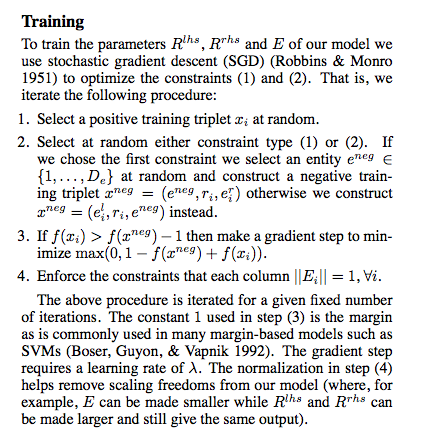
\includegraphics[width=\linewidth]{bordes_sgd.png}
  \caption{caption}
  \label{"waiting for reftex-label call..."}
\end{figure}



\end{document}
